\newcommand{\build}{\textit{build} }
\newcommand{\plugin}{``Plugin'' }
\newcommand{\plugins}{``Plugins'' }
\newcommand{\rsm}{``RSM'' }
\newcommand{\together}{``Together'' }

\begin{mainmatter}

	\chapter{Introduction}

\section{Présentation de l'entreprise d'accueil}
Créée en 2003 par Laurent Py et Bruno LEGEARD, la société LEIROS est spécialisée dans le test logiciel. Elle est issue du projet Smart Testing\texttrademark ~au LIFC\footnote{Laboratoire d'informatique de Franche-Comté}. L'objectif premier de LEIROS a été d'industrialiser le projet Smart Testing\texttrademark.  LEIROS a ensuite changé de nom pour devenir Smartesting en juin 2008. En septembre 2008, Smartesting ouvre sa filiale à Bangalore, en Inde. Smartesting compte environ trente-cinq personnes dont onze dans le service R\&D \footnote{Recherche et développement}.

\begin{figure}[!ht]
\centering
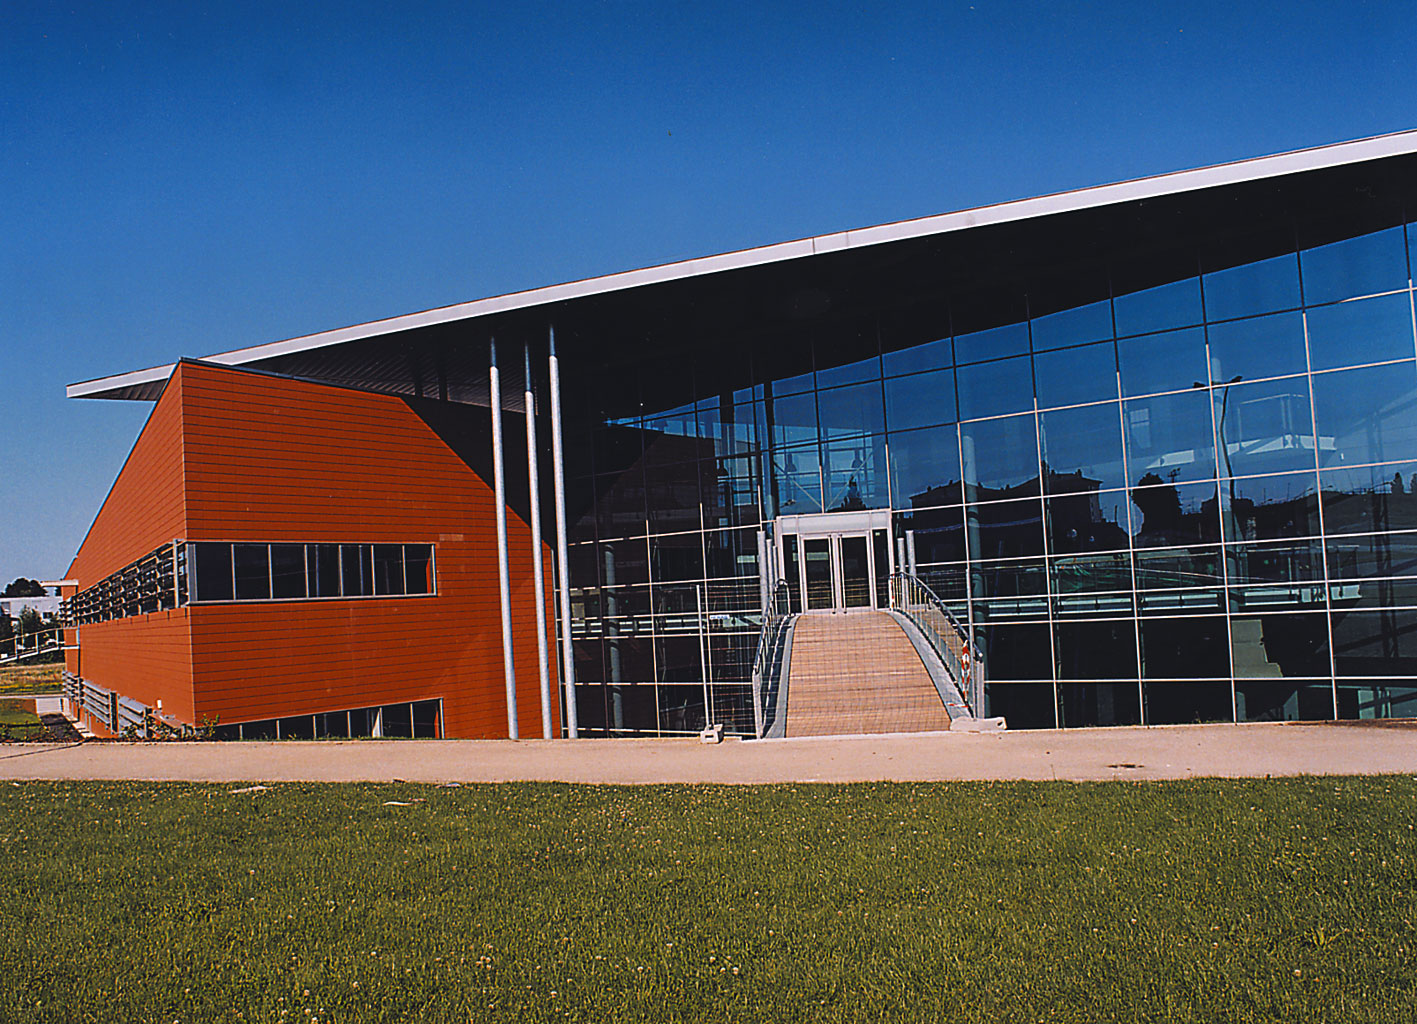
\includegraphics[width=.55\textwidth]{Illustrations/temis.jpg}
\caption{Centre Temis à Besançon}
\label{figure:temis}
\end{figure}

\subparagraph*{}
Smartesting est implantée dans différents points stratégiques. En France,le siège social ainsi que le centre R\&D sont à Besançon dans les locaux de l'hôtel d'entreprises TEMIS Innovation(cf. figure \ref{figure:temis} p.\pageref{figure:temis}). Ainsi la R\&D reste proche géographiquement de l'université et de la recherche qui y a lieu. À Paris et à Amsterdam aux Pays-Bas se trouvent les agences où travaillent les commerciaux et les avant-vente. Smartesting s'est implantée à Bangalore, en Inde où elle compte réaliser la moitié de son chiffre d'affaires en 2010 grâce au boom de l'offshore où le marché du test logiciel est en pleine expansion.

\subparagraph*{}
Smartesting développe dans le secteur grandissant du test logiciel. Ce marché devrait atteindre 13 milliards de dollars en 2010 (selon une étude de Gartner). Le test logiciel, en particulier le test fonctionnel devient une phase clé du développement logiciel. Des besoins très stricts pour les milieux bancaires par exemple obligent ces entreprises à faire appel à des ingénieurs et des architectes de test afin de concevoir les tests logiciels qui permettront par exemple de garantir la stabilité, la non regression et le bon fonctionnement de gros projets. Smartesting propose Test Designer, une solution de génération automatique de référentiels de test à plusieurs niveaux.

\begin{figure}[!ht]
\centering
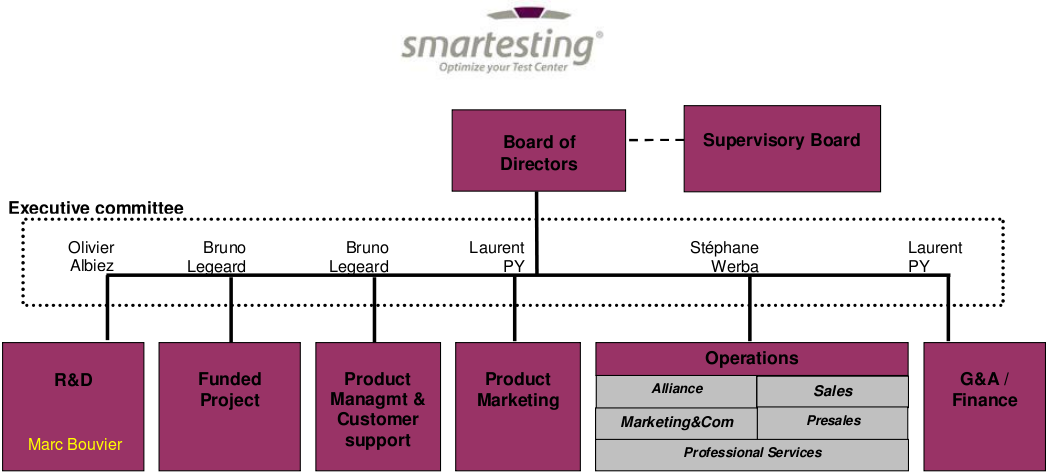
\includegraphics[width=\textwidth]{Illustrations/Organigramme_with_me.png}
\caption{Organigramme}
\label{figure:Organigramme de Smartesting}
\end{figure}

\subparagraph*{}
L'entreprise est organisée autour d'un directoire de trois personnes : Laurent PY, Bruno LEGEARD et Stéphane WERBA.Je travaille dans le service de R\&D{}\ de Smartesting.  L'équipe est composée de 11 ingénieurs dévelopeurs qui améliorent sans cesse le produit Test Designer ainsi que les connecteurs et les publishers y sont développés. L'équipe fonctionne autour de méthodes Agiles, en particulier eXtreme Programming. Ces sujets seront développés dans les sections qui vont suivre.

\pagebreak

\section{Test Designer}
La solution Test Designer permet de générer des référentiels de tests fonctionnels à partir de modèles UML pour le test/footnote{Model Based Testing}. Elle fait le lien entre la modélisation de tests et le management de tests.

%Figure 
\begin{figure}[!ht]
\centering
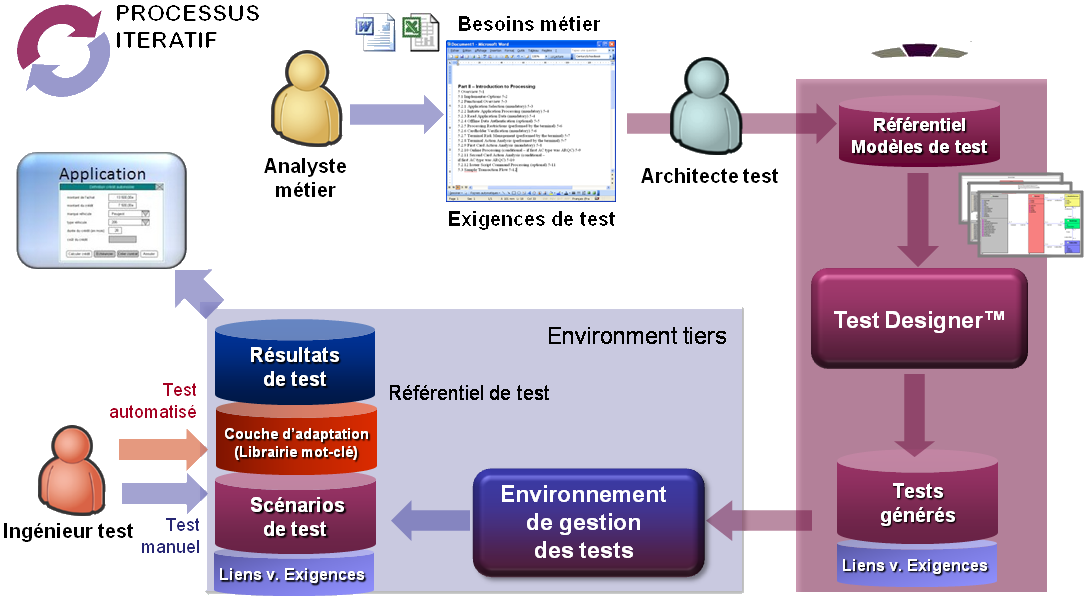
\includegraphics[width=\textwidth]{Illustrations/TheSolutionSmartesting.png}
\caption{La solution Smartesting}
\label{figure:La Solution Smartesting}
\end{figure}

\subparagraph*{}
La modélisation de tests se fait à l'aide de modeleurs UML basés sur Eclipse\footnote{Eclipse est une plateforme applicative sur laquelle peuvent se greffer des applications clientes sous forme de plugins(extensions)}. Les modeleurs supportés actuellement par Test Designer sont Borland Together 2008 et IBM Rational Software Modeler 7.0.5 \& 7.5. Il s'agit de modeleurs basés sur la plateforme Eclipse. Eclipse est une architecture de plugins qui communiquent les uns avec les autres pour former une application. C'est via ce mécanisme que Smartesting a développé deux plugins d'exportation de modèle pour les deux modeleurs précédemment cités.

\subparagraph*{}
Une fois le modèle de tests exporté il est utilisable par Test Designer pour générer automatiquement des référentiels de tests. Ces tests sont stockés dans un référentiel de test. Ces test pourront être publiés vers des evironnements tiers (HP Quality Center, tests JUnit, XML, Specifications pdf...).

\subparagraph*{}
Le processus de génération de tests de la solution Smartesting est un processus itératif. C'est à dire que si l'application déjà testée doit évoluée, la prise en compte des nouvelles fonctionnalités, ne générera pas un nouveau coût de génération des tests. 
Il suffit de modifier le modèle UML de spécifications via le modeleur, puis de générer les tests à nouveau (automatique). Ainsi les architectes de test gagnent un temps considérable à ne pas générer des test qui sont déja existants.

\subparagraph*{}
Traditionnellement la génération de tests est effectuée manuellement par un ingénieur de tests.

\section{Environnement de travail}
La première tâche qui m'a été confiée à mon arrivée fut d'installer mon poste de travail. Un ordinateur avec Ubuntu 8.10 m'a été confié et j'y ai installé IntelliJ Idea 8.0 (IDE\footnote{Environnement de développement intégré}), adapter quelques options de configuration au développement sur le projet Test Designer. Je me suis ensuite familiarisé pendant une semaine avec le code existant. La consigne était de ne demander d'aide de personne pendant une semaine. Au debut de la semaine qui suivit, je devais faire une compte rendu de ce que j'avais compris. Ce ``test'' permet en fait à l'équipe d'avoir un  marqueur sur la lisibilité du code source. Après cette phase d'apprentissage de l'existant, j'ai commencé à travailler sur des fonctionalités de Test Designer.

\subparagraph*{}
Le code source de Test Designer (le coeur de métier de Smartesting) est développée en JAVA avec un moteur de génération de tests qui s'appuie sur une approche prover (en c++). L'injection de dépendances est gérée par PICO. Une grande variété de bibliothèques sont utilisées telles que les google collections, JUnit, Mockito, JTidy, ou encore JYaml. Certaines ``boîtes à outils'' sont néanmoins développés en interne pour les besoins de la production. Les plugins dans les modeleurs utilisent l'architecture en plugin d'Eclipse pour s'y intégrer. En ce qui concerne les publishers, ils sont un fichier XML créé à partir du référentiel de tests. Ce fichier est ensuite exploité par le biais d'une API développée par l'équipe est distribuée aux clients lors de la livraison. Finalement l'API est aussi bien utilisée par les développeurs de l'équipe R\&D, les consultants de Smartesting que les clients finaux.
	
	\chapter{Le modeleur open source}

L'intégration d'un plugin Test Designer pour Papyrus a nécessité une phase d'exploration. Celle-ci a permis de mettre en évidence des correspondances entre les librairies RSM et Papyrus. A la suite de cette exploration, un certain nombre de décisions concernant la réorganisation de module en plugin a été planifié.

\subparagraph*{}
L'amélioration du \build a fourni une aide précieuse dans le déploiement d'autres plugins. 
Cela a contribué à la fragmentation en plugins.

\subparagraph*{}
Malgré les ressemblances au modeleur RSM, certaines spécificités ont du être développées pour le modeleur Papyrus.
A la suite de quoi, j'ai étudié le mécanisme de point d'extension d'Eclipse.

\section{Étude du modeleur Papyrus}

Cette partie traite de l'exploration menée sur le modeleur Papyrus.
Elle permet de mettre en évidence les actions à mener, pour créer un plugin exporter pour Papyrus.
Aux vues des premières constatations sur l'ensemble des plugins utilisés par le modeleur.
La ressemblance avec le modeleur RSM fut constatée.

\subparagraph*{}
Papyrus est un modeleur en cours de développement par le CEA\footnote{Commissariat à l'Energie Atomique}.
Il est actuellement livré dans sa version 1.11 mais la version 2 est en cours de développement.
Avec ce modeleur certaines fonctionnalités n'ont tout simplement pas été développées.

Pour étudier le modeleur Papyrus, j'ai téléchargé le code source du modeleur\footnote{Disponible sur https://speedy.supelec.fr/Papyrus/svn/Papyrus/core/releases/1.11.0/}.

\subparagraph{Fonctionnalités non fonctionnelles : }
\begin{itemize}
  \item Impossibilité de réaliser des transitions internes dans un diagramme d'état.
  \item Initialisation automatique des liens entres deux instances d'objet.
  \item Impossible de définir des stéréotypes manuellement.
\end{itemize}

\subparagraph{CEA :}
C'est un acteur majeur en matière de recherche, de développement et d’innovation, le CEA intervient dans trois grands domaines :
\begin{itemize}
  \item  l’énergie
  \item les technologies pour l’information et la santé
  \item la défense et la sécurité
\end{itemize}

\subsection{Points communs}

Les premières constatations du modeleur ont mis en évidence des points communs avec le modeleur RSM.
Papyrus utilise le même framework de stockage du modèle : Emf\footnote{Editing Modeling Framework}.

\subparagraph*{}
Lors de l'exploration, j'ai utilisé le plugin d'exportation d'RSM.
Cela m'a permis de montrer une grande compatibilité avec ce modeleur et la possibilité de réutiliser le code d'extraction d'un modèle RSM dans Papyrus.
Pour réutiliser ce code, j'ai envisagé de fragmenter le plugin ``RSM Exporter'', et créer un autre plugin ``Emf Exporter''.
Cela a pour but de garder uniquement le code spécifique à chaque modeleur dans leur plugin respectif.

\subparagraph*{}
Il n'y a toute fois pas que des points communs.

\subsection{Différences}

\subparagraph{Manque d'utilitaires :}
Comme Papyrus est un modeleur incomplet, il manque d'utilitaires qui permettent de faciliter l'exportation du modèle UML.
Dans RSM, il y a par exemple, une classe qui retourne la liste des modèles ouverts.
Ainsi à partir de celle-ci et du projet en cours de sélection, le modèle du projet sélectionné est récupéré.

\subparagraph*{}
Dans l'interface graphique quelque soit la version d'RSM, il faut ouvrir au moins un élément pour pouvoir accéder au modèle.
Comme on peut le voir sur la figure \ref{OpenProject} p.\pageref{OpenProject}, il y a une différence entre projet ouvert et fermé. 
Tant que le modèle n'a pas été chargé en mémoire, il est impossible d'en extraire les données pour les exporter vers ``Test Designer''. C'est une particularité du modeleur que n'a pas ``Together''.

\begin{figure}[!h]
\begin{center}
  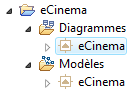
\includegraphics[scale=.7]{images/RsmOpenProject.png}
   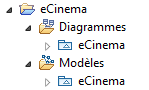
\includegraphics[scale=.7]{images/RsmOpenProject2.png}
  \caption{Projet non ouvert / Projet ouvert}
  \label{OpenProject}
\end{center}
\end{figure}

\subparagraph*{} 
En fait les données du projet RSM sont stockées dans un fichier ``emx''. 
Ce fichier est un document XMI\footnote{XML\footnote{Extensible Markup Language} Metata Interchange} utilisé par le framework Emf pour y stocker les données du modèle. 
Il s'agit d'un framework Java et un générateur de code pour les applications basées sur les modèles structurés. Il permet de prendre en compte toutes les informations contenues dans les diagrammes UML\footnote{Unified Modeling Language}.

\subparagraph{Edition du modèle :}
Quelque soit le modeleur, il existe une fonctionnalité dans l'exporter de modèle qui permet de définir un filtre sur des suites du modèle.
La particularité de cette propriété, est qu'elle est enregistrée dans le modèle UML.
Ainsi dans RSM, on utilise le framework de stockage des éléments UML pour y stocker une propriété supplémentaire sur l'élément suite.

\subparagraph*{} 
Le principe utilisé dans RSM  pour modifier le modèle, ne peut être utilisé de façon identique dans Papyrus. 
Le manque d'utilitaire empêche la réalisation simple du même procédé.
C'est à la suite de la découverte de cette différence que j'ai étudié la procédure d'édition du modèle d'RSM (paragraphe \ref{subsubsection:EditingDomaine} ''Edition du modèle UML d'RSM'' p.\pageref{subsubsection:EditingDomaine} ).

\subparagraph*{}
Parmi les fonctionnalités du plugin d'exportation seul deux fonctionnalités modifient l'état du modèle :
\begin{itemize}
  \item Le filtre sur les suites. 
  		Une suite est un package UML, qui spécifie l'état initial du modèle de génération de tests.
  \item L'éditeur OCL\footnote{\textit{O}bject \textit{C}onstraint \textit{L}anguage}. Il s'agit d'un plugin développé pour RSM qui permet d'éditer plus facilement une garde et un effet sur une transition dans un diagramme d'état. Il offre notamment la complétion\footnote{Complément automatique} et la coloration syntaxique\footnote{Repésentation des mots-clés sous une police différente pour les mettre en évidence}.
\end{itemize}

\subsection{Structure d'un projet Papyrus}

L'étude de la struture du projet Papyrus a aidé à la récupration du modèle.

\subparagraph*{}
Comme on peut l'observer sur la figure \ref{PapyrusProject} p.\pageref{PapyrusProject}, un projet Papyrus est composé de deux fichiers. Le fichier \texttt{.project} appartient à la plateforme Eclipse.
\begin{itemize}
  \item Fichier \texttt{.di2} : Contient les données graphiques des diagrammes de celui-ci. Il s'agit d'un format Xmi comme RSM mais avec un élément \texttt{<di2>} spécifique.
  \item Fichier \texttt{.uml} : Celui-ci contient les données du modèle UML enregistrées au format Emf (XMI).
\end{itemize}

\begin{figure}[!h]
\begin{center}
  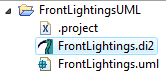
\includegraphics[scale=1]{images/PapyrusProject.png}
  \caption{Fichiers d'un projet Papyrus}
  \label{PapyrusProject}
\end{center}
\end{figure}

\subparagraph*{}
Pour récupérer les données du modèle Emf, il faut utiliser les utilitaires d'Emf pour charger le fichier \texttt{.uml} afin d'en extraire les données UML. C'est à partir de ces données que l'exportation du modèle Emf vers ``Test Designer'' est effectuée.

\subparagraph*{}
A partir de ces données est-il possible de les modifier ?

\subsection{Edition du modèle UML}\label{subsubsection:EditingDomaine}

En l'état, un modèle Emf peut être modifié par des méthodes de modification du modèle.
Hors ce procédé ne peut fonctionner correctement.
Sur un modèle Emf, il est donc obligatoire de passer par un mécanisme centralisé d'édition du modèle.
Ce mécanisme a pour but de modifier le modèle de façon transactionnel.
Toute modification de la propriété d'un élément est réalisée de façon atomique.
Si jamais la modification devait échouée en cours de transaction, le modèle reviendra à l'état précédant.

\subparagraph*{}
Dans Emf, il est appelé ``EditingDomain''.
Les modeleurs sont libres de l'utiliser comme ils le souhaitent.
Il faut de toute façon pouvoir récupérer l'``editingDomain'' des modèles ouverts.
C'est ce que permet de faire RSM via un utilitaire.

\subsection{Récupération d'un modèle}

Papyrus utilise le mécanisme d'adaptation d'Eclipse.
Ce mécanisme permet de retourner un objet instancié par un éditeur ou un objet \texttt{IAdaptable}.
Dans Eclipse, les objets adaptables sont par exemple, les éditeurs et les ressources du projet.

\begin{figure}[!ht]
	\begin{minipage}[c]{0.6\linewidth}
 		\begin{center}
	  		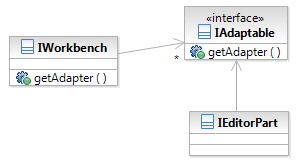
\includegraphics[scale=.6]{images/DiagAdapter.png}
	  		\label{DiagramClassEditor}
	  		\caption{Diagramme de classe d'un éditeur}
		\end{center}
 	\end{minipage}\hfill
 	\begin{minipage}[c]{0.4\linewidth}
 		Tous les éditeurs implémentent \texttt{IEditorPart}. Ainsi tous les éditeurs qui surchargent la méthode  \texttt{getAdapter(Class class)} de l'interface \texttt{IAdaptable} permettent de retourner un objet de la classe passée en paramètre.
 	\end{minipage}
\end{figure}

\subparagraph*{}
C'est ce mécanisme qui a été utilisé dans Papyrus pour récupérer le modèle ouvert.
Exemple, à partir du ``Workbench'' qui est l'espace de travail d'Eclipse. 
Il est possible de demander le modèle UML en faisant : 
\begin{small}
\begin{verbatim}Model theModel = IWorkbench.getAdapter(org.eclipse.uml2.uml.Model.class)\end{verbatim}
\end{small}
Autre exemple si l'on souhaite récupérer un ``editingDomain'', il faudra utiliser :
\begin{small}
\begin{verbatim}EditingDomain editingDomain = IWorkbench.getAdapter(EditingDomain.class)\end{verbatim}
\end{small}
Il y a toute fois un inconvénient à cette solution. Si aucun éditeur n'est ouvert, il n'y a pas de modèle récupérable.

\subsection{Les stéréotypes}

Les stéréotypes sont une fonctionnalité qui a posé problème.
Cette partie a pour but d'expliquer, à quoi ils servent.

\subparagraph*{}
Les stéréotypes sont des propriétés des objets UML, ils permettent de spécifier le comportement de ceux-ci. 
Dans notre cas, d'autres ont été ajoutés pour permettre de spécifier par exemple le comportement d'une opération (figure \ref{stereotype} p.\pageref{stereotype}). 
En spécifiant ``observation'' sur l'opération ``myOperation'' cela signifie que la post condition qui détermine l'état final après exécution de l'opération, ne modifie pas l'état du modèle. 
Et celle-ci doit retourner une valeur. 
Concernant la vérification des stéréotypes, cela est effectué via un contrôle d'erreur au moment de l'exportation du modèle. 
La post-condition est une propriété de l'opération écrit en OCL.

\subparagraph{}
Dans RSM les stéréotypes sont gérés par une extension spécifique au modeleur, qui permet d'ajouter d'autres stéréotypes que ceux standards (interface, abstract, enumeration, \ldots), par exemple : 
\begin{itemize}
  \item observation
  \item setup
  \item teardown
\end{itemize}
Une extension est un mécanisme qui permet d'étendre les fonctions du modeleur à condition que celui-ci l'accepte.

\begin{figure}[!h]
\begin{center}
  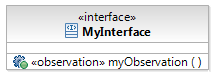
\includegraphics[height=2cm]{images/stereotype.png}
  \caption{Exemple de stéréotype dans RSM}
  \label{stereotype}
\end{center}
\end{figure}

\subparagraph*{}
Quel bilan peut on faire à partir des constations suivantes ?

\subsection{Résultat}

Le bilan de cette étude montre en effet que Papyrus est proche d'RSM.
Toute fois, il est nécessaire que la fragmentation soit effectuée avant de factoriser le code commun pour les deux modeleurs.

Maintenant, concernant les différences et les problèmes constatés en réalité, ceux-ci ne posent aucun problème.
Il y a en effet dans les objectifs de jalon suivant, une modification sur la gestion des suites qui doit supprimer les modifications du modèle. 
Et Smartesting souhaite d'autre part ne plus rien enregistrer dans le modèle.

\subparagraph*{}
Pour l'éditeur OCL, il s'agit d'un plugin qui n'est destiné qu'à RSM.
En sachant que Papyrus n'a pas besoin d'éditer plus facilement une ``garde'' et un ``effet'' car cela l'est suffisamment\footnote{Trois cliques de souris avec Papyrus contre une dizaine avec RSM}.

\subparagraph*{}
Pour la récupération du modèle, il a été fait le choix de récupérer le modèle à partir du fichier \texttt{.uml}.
La manière qui utilise le mécanisme d'adaptation d'Eclipse ne correspond pas à l'attente fonctionnelle du client XP.

\section{Problèmes rencontrés}

Durant l'exploration, un certain nombre de problèmes et de questions ont été soulevés.
Pour certains, il s'agit tout simplement de l'incapacité du modeleur à modéliser pour le test.
Dans d'autres cas, il s'agit d'un fonctionnement qui engendre des erreurs dans le modèle.

Liste des problèmes :
\begin{itemize}
  \item Problème sur les instances de lien dans le modèle
  \item Ajout de nouveaux stéréotypes
  \item Gestion des ranges sur les entiers
  \item Problème d'extraction des commentaires
\end{itemize}

\subsection{Problème sur les instances de lien dans le modèle}

Lorsque l'on souhaite créer un lien entre deux instances dans Papyrus, une erreur non explicite est détectée au moment de l'exportation du modèle.
Après une recherche de la cause possible de cette erreur, nous avons fini par en déduire la cause d'une mauvaise construction du lien dans Papyrus. 
Nous avons constaté que les slots du lien en question, ne sont pas créés automatiquement contrairement à ceux du modeleur RSM.

\subparagraph*{}
La figure \ref{ProblemLink} p.\pageref{ProblemLink} est une capture du modeleur Papyrus qui met en évidence le problème lié à la création de lien d'instance (1).
On peut voir entouré en rouge (2) que les slots ne sont pas initialisés. Pour cela, il faut les initialiser manuellement pour arriver au résultat encadré en orange (3).

\begin{figure}[!ht]
\begin{center}
  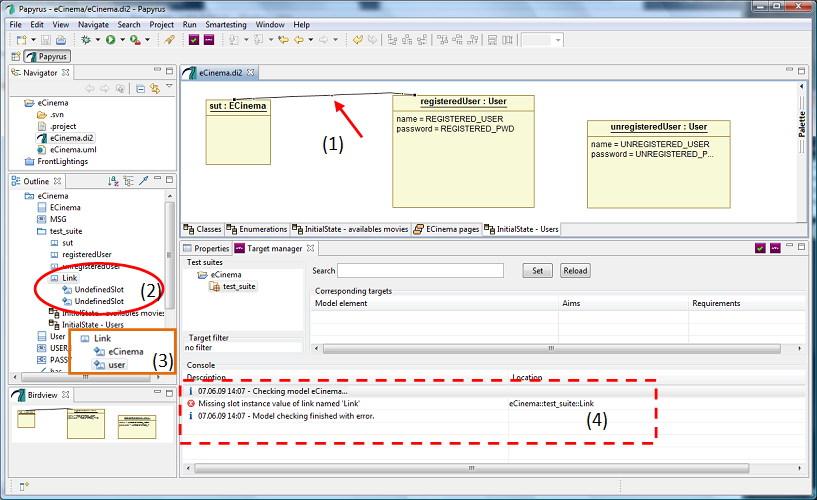
\includegraphics[width=.9\linewidth]{images/Papyrus.png}
  \caption{Modeleur Papyrus - Problème sur le lien entre instances}
  \label{ProblemLink}
\end{center}
\end{figure}

\subparagraph*{}
C'est via ce problème que nous avons mis en évidence un manque de clarté de certains messages d'erreurs pas assez explicites du genre \texttt{NullPointerException} ou \newline \texttt{IndexOutOfBoundException} qui ont été corrigés pour donner le résultat dans l'encadré en pointillés rouges (4) figure \ref{ProblemLink} p.\pageref{ProblemLink}.

\subsection{Gestion des ranges sur les entiers}

La fonctionnalité de range d'entier est réalisée à partir d'un point d'extension spécifique à RSM. Cette fonctionnalité n'existe pas dans le modeleur Together. 
Cette fonctionnalité offre la possibilité de paramétrer graphiquement le range représentant un entier.
Lors de la modélisation pour les tests, les valeurs des paramètres d'entrée d'une opération génèrent autant de cas de tests que de combinaisons de valeurs possibles de ces paramètres. 
Pour diminuer le nombre de tests, on utilise des ranges sur les entiers.
A noter qu'il est possible de limiter les valeurs prises par le paramètre entier, via la pré-condition de l'opération.
Ce qui ne constitue donc pas un problème pour Papyrus.

\subsection{Problème d'extraction des commentaires}

La gestion des commentaires dans RSM et Papyrus est différente.
Il faut donc gérer cette fonctionnalité comme spécifique dans les deux modeleurs.
La récupération est bien effectuée sur le même objet EMF, mais un filtre pour RSM est appliqué pour récupérer la documentation texte ou HTML saisie par l'utilisateur ne correspond pas pour Papyrus.
Il est donc nécessaire de développer spécifiquement deux extracteurs de commentaires, un pour RSM et un pour Papyrus.

\subsection{Comment est géré le spécifique de chaque modeleur ?}

L'adaptation spécifique à chaque modeleur est réalisée au moment du clique sur le bouton ``check'' et ``export''. 
C'est l'endroit de plus haut niveau où il est permis de spécifier les objets spécifiques au modeleur.
Exemple : 
\begin{verbatim}
EclipseTranslatorUtils.translateAndCheckModel(
                selection.project,
                selection.umlModel,
                new RsmModelExtractor(),
                new RsmTestSuiteTranslator(),\ldots);
\end{verbatim}
Sur l'exemple ci-dessus, la méthode ``translateAndCheckModel'' réalise l'extraction du modèle. 
Celle-ci prend en paramètre le projet sélectionné et le modèle Emf parce qu'il s'agit d'RSM. 
Pour \together, c'est un objet \texttt{Emfapi}.
Ensuite la méthode d'extraction est réalisée spécifiquement par passage de l'utilitaire d'extraction ``RsmModelExtraction'' en paramètre.

\subparagraph{}
Pour pouvoir réutiliser le code d'RSM pour l'adapter à Papyrus nous avons généralisé l'extracteur d'RSM en ``EmfModelExtractor'' avec spécification de la méthode de récupération des descriptions dans un driver. Ce qui donne :
\begin{verbatim}
return EclipseTranslatorUtils.translateAndCheckModel(
                selection.project,
                selection.umlModel,
                new EmfModelExtractor(new RsmExtractorDriver()),
                new EmfTestSuiteTranslator(new RsmExtractorDriver()),
\end{verbatim}
En réalisant cette généralisation, il est possible d'ajouter des traitements spécifiques dans le driver d'extraction.


	
	\section{La plateforme Eclipse}

Avant de parler de fragmentation en plugins, il est important de définir le fonctionnement d'Eclipse.

\subsection{Historique}

Créée en 2001, le but du projet Eclipse était de fournir un socle pour la création d'environnements de développement.
\subparagraph*{}
En 2004, lors du lancement d'Eclipse RCP\footnote{Rich Client Platform}, l'objectif du projet a été étendu pour prendre en compte l'utilisation du framework Eclipse par des applications clientes.
Au départ, Eclipse était conçu pour créer un environnement de développement Java autour duquel aurait été construit d'autres applications.
Finalement, la base est conçue comme un framework utilisable pour des développements d'applications clientes dîtes riches.

\subsection{Principe}

Eclipse est une plateforme composée de plugins qui interagissent les uns avec les autres (figure \ref{PlatformEclipse} p.\pageref{PlatformEclipse}).
La plateforme Eclipse est fournie avec un framework minimaliste appelé ``Runtime''. Contrairement à une application extensible qui est composée d'une gros framework commun.
Autour de ce framework d'autres plugins sont déployés afin de permettre la création d'une application riche.
Exemple : 
\begin{itemize}
  \item SWT : création de composants graphiques
  \item JFace : création de composants plus riches basés sur SWT
  \item Workbench : gestion de l'environnement de travail (menu, action, \ldots)
\end{itemize}

Cette plateforme basée sur l'extensibilité est réalisée grâce au mécanisme de points d'extension.

\begin{figure}[!h]
\begin{center}
  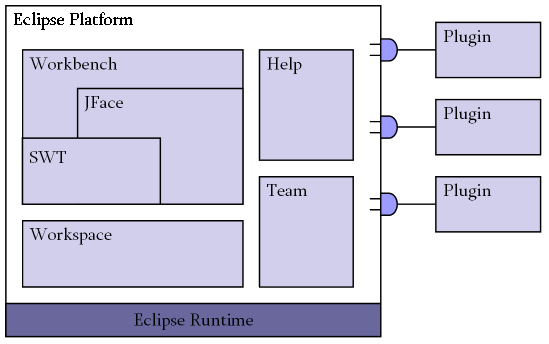
\includegraphics[scale=.55]{images/archi_eclipse_platform.png}
  \caption{Diagramme représentant une plateforme Eclipse}
  \label{PlatformEclipse}
\end{center}
\end{figure}

\subparagraph*{}
Le framework de base sert de conteneur pour les extensions.
Toutes les fonctionnalités sont développées dans des <<plug-in>> (Bundles).
Cela offre l'avantage d'être ouvert et transparent. 
Il est par exemple plus facile de remplacer une fonctionnalité par une autre.

\subparagraph*{}
Une application basée sur Eclipse utilise le registre d'extension et les services OSGI\footnote{Open Services Gateway initiative}.
Ce standard permet de gérer les dépendances de plugin et l'extensibilité de l'application.
Il évite aussi le couplage des modules Java.
Pour modulariser l'application, il suffit d'utiliser les ``features'' Eclipse.

\subparagraph*{}
Une feature Eclipse permet de déployer des plugins différemment suivant le client ou suivant la plateforme cible.

\subsection{Déploiement d'un plugin sur une plateforme Eclipse}

La plateforme Eclipse implémente le mécanisme de mise à jour d'une application que l'on retrouve sur quasi tous les logiciels.
Dans Eclipse un plugin peut être déployé par un ``update-site''.

\subparagraph*{}
En réalité, un ``update-site'' déploie des ``features'' composées de ``plugins'' (figure \ref{figure:EclipsePlatformDeploiement} p.\pageref{figure:EclipsePlatformDeploiement}).
Le mécanisme d'installation, vérifie en fonction des plugins requis par la feature à installer si la plateforme Eclipse les possède.
En cas d'échec les plugins ne sont pas installés.

\begin{figure}[!h]
\begin{center}
  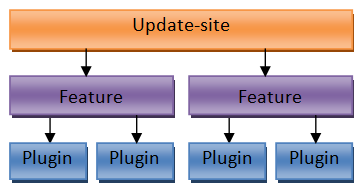
\includegraphics[scale=.55]{images/archi_eclipse_deploiement.png}
  \caption{Architecture de déploiement d'un plugin sur la plateforme Eclipse}
  \label{figure:EclipsePlatformDeploiement}
\end{center}
\end{figure}

\subsection{Structure}

Cette partie définie la composition des différents éléments Eclipse : Plugin et feature.

\subsubsection{Feature}

Une feature est gérée par un fichier \texttt{feature.xml} qui contient au format XML, la liste des plugins composants la fonctionnalité.

\subsubsection{Plugin}

L'administration des plugins est gérée par OSGI, qui utilise le fichier \texttt{MANIFEST.MF} contenu dans la structure du plugin. 
C'est ce fichier qui permettra de gérer les dépendances de plugins.

Quant à Eclipse, la plateforme utilise entre autre le fichier \texttt{plugin.xml}.
Ce fichier contient les données XML de construction de l'interface utilisateur.
On peut y déclarer des actions, des menus, des vues, des éditeurs, \ldots

\subsubsection{OSGI}\label{OSGI}

Eclipse utilise le framework OSGI, qui permet de gérer le chargement des classes, l'administration des plugins et les dépendances entre eux. 
Pour généraliser, ce framework Java gère le cycle de vie d'une application, les services, un environnement d'exécution et des modules.

	
	\section{Le build}\label{section_build}

La tâche de \textit{build} concerne un processus automatisé qui permet de réaliser des opérations de compilation et de déploiement pour construire par exemple les versions distribuées par Smartesting à ses clients.
Ce processus a été modifié afin de pouvoir fragmenter les plugins existants.

\subparagraph*{}
Au début du stage, le \textit{build} permettait de déployer deux plugins pour les deux modeleurs RSM et Together.
L'objectif fut donc d'entreprendre la modification de celui-ci pour faciliter la création et le déploiement d'autres plugins, en vue de progressivement passer des modules Java en plugins pour Eclipse.

\begin{figure}[!h]
\begin{center}
  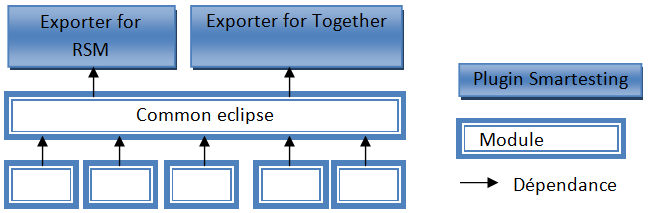
\includegraphics[scale=.6]{images/AvantBuild.png}
  \caption{Projet avant amélioration du \build}
  \label{AvantAmeliorationBuild}
\end{center}
\end{figure}
\ \\
Sur la figure \ref{AvantAmeliorationBuild} p.\pageref{AvantAmeliorationBuild}, les modules de type plugin sont gérés spécifiquement pour être déployés via un ``update-site''.

\subsection{Objectifs}

L'un des objectifs de l'amélioration du \build est de pouvoir créer des plugins Eclipse et les déployer.
La stratégie doit permettre de différencier plusieurs types de modules :
\begin{itemize}
  \item Update-site
  \item Feature
  \item Plugin (Smartesting)
  \item Module Java
  \item Librairie Java
  \item Plugin Eclipse
\end{itemize}
\ \\
La figure \ref{AmeliorationBuild} p.\pageref{AmeliorationBuild} montre l'amélioration apportée au \build. 
On peut remarquer la diversité des types de modules et des relations de dépendance.
La gestion des dépendances qui est aussi un enjeu puisqu'il faut que le \build construise les fichiers de configuration des plugins.

\begin{figure}[!h]
\begin{center}
  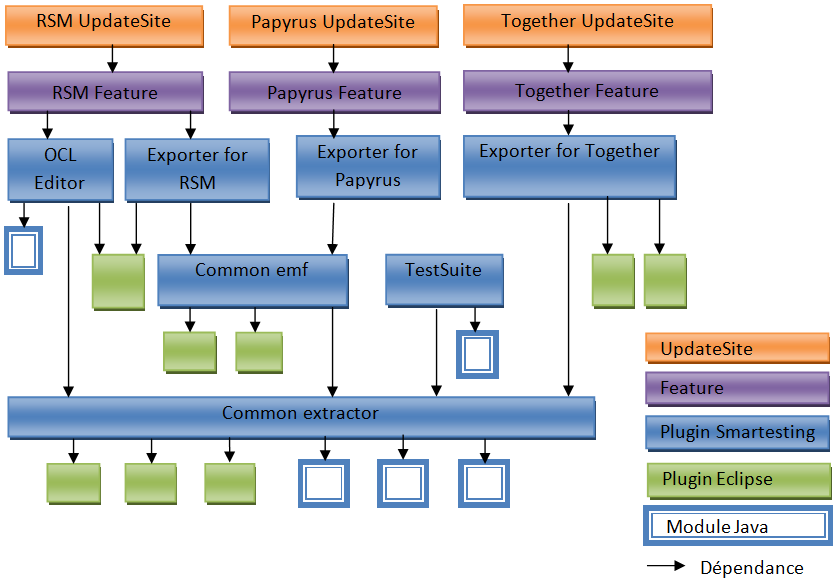
\includegraphics[height=7.5cm]{images/AmeliorationBuild.png}
  \caption{Projet après amélioration du \build}
  \label{AmeliorationBuild}
\end{center}
\end{figure}

\subsection{Fonctionnement du \build}

Le développement de la solution Smartesting est réalisé grâce à l'éditeur Java, IntelliJ\footnote{IntelliJ ou IDEA} de JBrain.
Il s'agit d'un éditeur payant dont le fonctionnement est proche de l'éditeur Java fonctionnant sous Eclipse.
Cet éditeur offre de nombreuses fonctionnalités qui rendent le développement plus facile.

\subparagraph*{}
Le \build mis en place par Smartesting, utilise les fichiers d'IntelliJ pour gérer les dépendances entre les modules.
Il y a donc une tâche \textit{ant} qui a été développée par Smartesting pour réaliser cela.

\subsubsection{Génération du manifest :}

La génération du manifest du plugin a été effectuée à partir d'un fichier manifest maintenu par le programmeur. 
Il est situé dans les sources du module plugin d'IntelliJ.
On y trouve la description du plugin et certains paramètres.
A l'intérieur de ce fichier, la version, le nom et les librairies Java sont générés automatiquement.

Exemple :
\tiny
\begin{verbatim}
Manifest-Version: 1.0
Bundle-ManifestVersion: 2
Bundle-Name: Exporter Plug-in
Bundle-SymbolicName: @plugin.identifier@;singleton:=true
Bundle-Version: @plugin.version@
Bundle-Vendor: SMARTESTING
Bundle-RequiredExecutionEnvironment: J2SE-1.5,
 JavaSE-1.6
Bundle-Classpath: .@plugin.runtime.manifest@
Require-Bundle: com.ibm.xtools.modeler;visibility:=reexport,
 com.ibm.xtools.modeler.ui;visibility:=reexport,
 \ldots
 com.smartesting.eclipse.emf;visibility:=reexport,
 com.smartesting.testsuite
Bundle-Activator: com.smartesting.ltd.eclipse.common.plugin.SmartestingPlugin
Bundle-Localization: plugin
Bundle-ActivationPolicy: lazy
Export-Package: com.smartesting.ltd.eclipse.rsm7.testsuite,
 com.smartesting.ltd.eclipse.rsm7.translator.extractor
\end{verbatim}
\normalsize

Dans cette exemple on y retrouve encadré par les @ les informations générées automatiquement.
Les autres informations sont spécifiques à chaque plugin.

\subparagraph*{}
Résultat de la génération :
\tiny
\begin{verbatim}
Manifest-Version: 1.0
Bundle-ManifestVersion: 2
Bundle-Name: Exporter Plug-in
Bundle-SymbolicName: com.smartesting.rsm.exporter;singleton:=true
Bundle-Version: 1.0.0.44657
Bundle-Vendor: SMARTESTING
Bundle-RequiredExecutionEnvironment: J2SE-1.5,
 JavaSE-1.6
Bundle-Classpath: .,
 lib/commons-lang-2.3.jar
Require-Bundle: com.ibm.xtools.modeler;visibility:=reexport,
 com.ibm.xtools.modeler.ui;visibility:=reexport,
 \ldots
 com.smartesting.eclipse.emf;visibility:=reexport,
 com.smartesting.testsuite
Bundle-Activator: com.smartesting.ltd.eclipse.common.plugin.SmartestingPlugin
Bundle-Localization: plugin
Bundle-ActivationPolicy: lazy
Export-Package: com.smartesting.ltd.eclipse.rsm7.testsuite,
 com.smartesting.ltd.eclipse.rsm7.translator.extractor
\end{verbatim}
\normalsize

	
	\section{Création d'un point d'extension Eclipse}\label{section_build}

Pour introduire des fonctionnalités spécifiques à un modeleur, j'ai étudié la possibilité d'utiliser un point d'extension d'Eclipse pour gérer les parties spécifiques du modeleur.

\subsection{Principe}

Le principe d'un point d'extension est le suivant. 
Eclipse est une grosse boîte sur laquelle on peut se brancher, mais pas seulement (cf. figure \ref{extension_point}).
Il s'agit aussi de plusieurs centaines de petites boîtes reliées les unes aux autres qui peuvent être connectées par un plugin pour le modeleur Papyrus. 
Les plug-ins ou (bundles) fournissent des points d'extensions.

\subparagraph*{}
Il faut imaginer qu'il s'agit d'une multiprise de courant où l'on peut brancher autant de connexions (extensions) que ne peut supporter la multiprise (un point d'extension).

\begin{figure}[!ht]
\begin{center}
  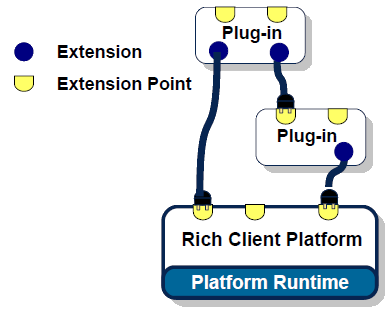
\includegraphics[scale=.5]{images/extension_point.png}
  \caption{Fonctionnement d'un point d'extension}
  \label{extension_point}
\end{center}
\end{figure}
\ \\
La première chose effectuée au moment du chargement d'un plugin, c'est les scans des metadata de tous les plugins, soit le fichier \texttt{plugin.xml}. 
Ceci n'étant effectué uniquement si les informations dans le cache d'Eclipse ne sont plus à jour, corrompues ou forcées (option -clean).

\subparagraph*{}
Si on exploite correctement les points d'extensions, il est possible de construire une interface graphique sans charger le plugin avec juste les metadata. 
Charger un plugin prend évidement de la mémoire et allonge le temps de démarrage d'Eclipse.

\subparagraph{Que se passe t'il lorsqu'un point d'extension est chargé ?}
Tout d'abord le fournisseur d'un point d'extension déclare celui-ci au registre d'extension.
Ensuite chaque plugin utilisant une extension s'identifie auprès du registre d'extension. Ces deux tâches sont automatiques, elles sont réalisées à partir du contenu des metadata (\texttt{MANIFEST.MF} et \texttt{plugin.xml}).

A partir de là, le fournisseur du point d'extension peut demander à instancier la classe déclarée par l'utilisateur du point d'extension (cf. diagramme de \ref{extension_point_sequence} p. \pageref{extension_point_sequence}).

\begin{figure}[!ht]
\begin{center}
  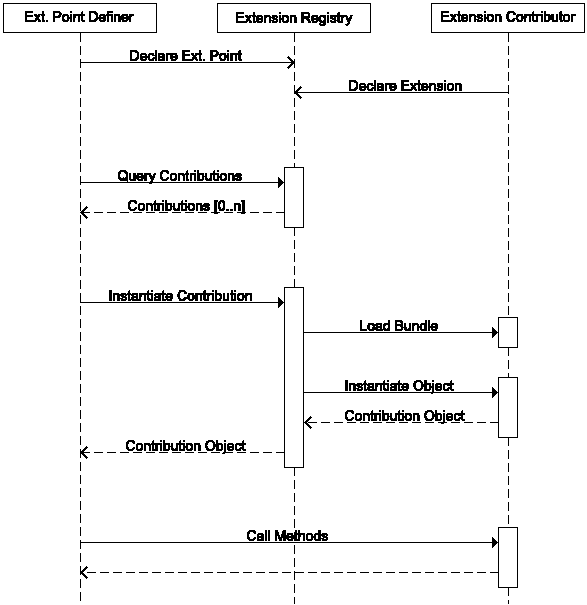
\includegraphics[scale=.7]{images/extension_sequense_diagram.png}
  \caption{Diagramme de séquence de l'enregistrement d'un point d'extension}
  \label{extension_point_sequence}
\end{center}
\end{figure}

\subparagraph{Précautions :}
Si un point d'extension est déclaré pour fournir une classe implémentant une interface I dans le plugin A. 
L'interface I doit être fournie par le plugin A déclarant le point d'extension.
Chaque plugin possède son propre environnement d'exécution\footnote{ClassLoader pour les programmeurs Java} (cf .\ref{OSGI} p.\pageref{OSGI}).
Ce qui signifie que la classe doit implémenter l'interface I du même environnement d'exécution (plugin A).
Même chose pour le type de retour des fonctions et ses paramètres, eux aussi doivent appartenir au même environnement d'exécution.

\subparagraph*{}
C'est a cette occasion que l'on utilise l'exportation de package dans le \texttt{MANIFEST.MF} via la propriété ``Export-Package''. Cette propriété permet de rendre visible par un autre plugin les classes contenues dans un package cible.

\subparagraph*{}
Avec ce mécanisme, il faut faire attention aux différents espaces de chargement des classes\footnote{ClassLoader}. Exemple : le plugin A propose le point d'extension \newline ``com.smartesting.core.extractor'' qui permet de définir une classe qui implémente l'interface  ``com.smartesting.extractor.Extractor'' via l'élément ``class''. Le plugin B utilise le point d'extension  ``com.smartesting.core.extractor'' avec comme classe \newline ``mon.plugin.extractor.MyExtractor''.

\subsection{Mise en \oe uvre}\label{subsection:MiseEnOeuvre}

Ce paragraphe explique le moyen de mise en \oe uvre d'un point d'extension pour gérer un extracteur de modèle spécifique au modeleur Papyrus. (A noter que les \ldots des exemples correspondent à un chemin de package).

\subsubsection{Etape 1 : Créer un point d'extension}

Il faut tout d'abord déclarer un point d'extension dans le plugin \texttt{Common Extractor} puisque tous les plugins d'export en dépendent.

Ensuite le point d'extension est définie dans le fichier \texttt{ModelExtractor.exsd}.
Puis on déclare dans le fichier \texttt{plugin.xml} le point d'extension :

\setlength\abovecaptionskip{0.25ex}
\setlength\belowcaptionskip{0.25ex}

\begin{figure}[H]
\centering
\begin{lstlisting}[language=XML]
<plugin>
	<extension-point id="ModelExtractor" 
		name="com.smartesting.eclipse.core"
	schema="schema/ModelExtractor.exsd"/>
</plugin>
\end{lstlisting}
\caption{Extrait du fichier \texttt{ModelExtractor.exsd} dans le plugin ``Common extractor''}
\end{figure}

Ensuite le fichier \texttt{Modelextractor.exsd} est configuré afin de permettre la déclaration de l'utilisation de l'extension comme ceci :
\begin{figure}[H]
\centering
\begin{lstlisting}[language=XML]
<extension point="com.smartesting.eclipse.core.ModelExtractor">
  <ModelExtractor
	  class="...PapyrusModelExtractor"/>
</extension>
\end{lstlisting}
\caption{Extrait du fichier \texttt{plugin.xml} du plugin ``Papyrus extractor''}
\end{figure}
Dans l'exemple précédent, l'attribut ``class'' permet de définir la classe qui permettra de rendre le service. 
Il a été choisi que la classe \texttt{PapyrusModelExtractor} devrait implémenter l'interface ``ModelExtractor''. 

\subsubsection{Etape 2 : Utiliser le point d'extension}

Pour utiliser les données du point d'extension, il faut passer par la plateforme Eclipse et interroger l'\texttt{ExtensionRegistry}\footnote{Platform.getExtensionRegistry()}. Grâce à ce service, nous pouvons récupérer l'instance de l'interface \texttt{ModelExtractor} qui sera \texttt{PapyrusModelExtractor}.

\subsubsection{Etape 3 : Exporter les classes dépendantes}

La dernière étape mais non des moindres, doit permettre de rendre visible depuis un autre plugin l'interface \texttt{ModelExtractor} dont \texttt{PapyrusModelExtractor}.
Pour cela, on ajoute la ligne suivante dans le fichier \texttt{MANIFEST.MF} du plugin ``Common extractor'' :
\begin{figure}[H]
\centering
\begin{verbatim}Export-Package: . . .ModelExtractor\end{verbatim}
\caption{Fichier \texttt{MANIFEST.MF} du plugin ``Common extractor''}
\end{figure}

\begin{figure}[!ht]
\begin{center}
  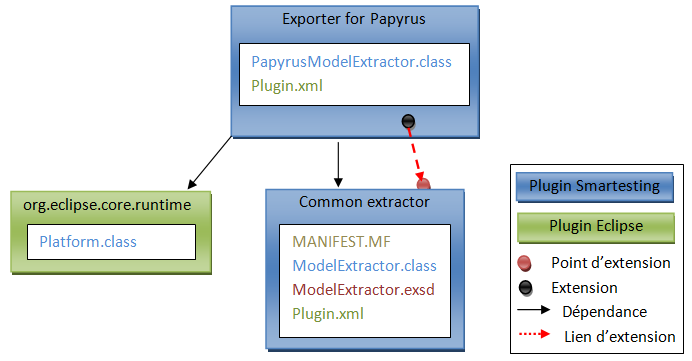
\includegraphics[scale=.5]{images/UsePapyrusExtensionPoint.png}
  \caption{Mise en \oe vre d'un point d'extension pour extraire le modèle UML}
  \label{figure:UsePapyrusExtensionPoint}
\end{center}
\end{figure}

La figure \ref{figure:UsePapyrusExtensionPoint} p.\pageref{figure:UsePapyrusExtensionPoint} montre l'infrastructure des plugins pour la mise en place du mécanisme de point d'extension.
\begin{description}
  \item [Le plugin ``Common extractor''] contient le fichier manifest dans lequel est déclaré visible la classe \texttt{ModelExtractor}.
Le fichier \texttt{ModelExtractor.exsd} contient la déclaration du point d'extension, son nom, sa structure XML. \texttt{Plugin.xml} contient la déclaration du fichier \texttt{ModelExtractor.exsd}.

\item [Le plugin ``Papyrus extractor''] contient un manifest contenant la dépendance avec ``Common extractor'', la classe spécifique d'extraction du modèle appelé \newline \texttt{PapyrusModelExtractor} et le fichier \texttt{plugin.xml} pour déclarer l'utilisation du point d'extension.
\end{description}

\subsection{Avantages /inconvénients}

La mise en place du mécanisme d'un point d'extension est simple à mettre en place et offre des résultats rapides.
Il faut éviter le piège sur le problème d'environnement d'exécution différent des plugins.

\subparagraph*{}
Il y a cependant, un problème lié à l'environnement d'Eclipse, qui utilise des variables globales comme ``Platform'' qui empêchent la réalisation de tests unitaires simples. 
La solution est d'abstraire la plateforme Eclipse pour pouvoir tester le mécanisme.

	
	\section{Synthèse}
	
	Le cheminement logique du travail réalisé fut, l'exploration du modeleur Papyrus.
	A la suite de quoi, la fragmentation du plugin RSM pour extraire le code commun avec Papyrus.
	La fragmentation a été freinée par l'amélioration du \build nécessaire à la mise en \oe uvre d'une architecture en plugin.
	Et pour finir, la création d'un point d'extension a permis de régler un problème de dépendance pour faire du spécifique.
	
	\subparagraph*{}
	Quoi qu'il en soit, toutes ces actions ont été menées avec succès.
	Et il ne reste plus qu'à en tirer les conclusions du stage qui s'imposent.
	
	\chapter{Conclusion}

Ce chapitre est la conclusion de tout le travail réalisé dans l'équipe R\&D de Smartesting.
C'est aussi, la conclusion d'un challenge personnel de reprise d'étude après cinq années passées dans la vie active.
Et pour finir, c'est l'occasion de dire, la chance que j'ai d'entrer dans l'équipe Smartesting.

\section{Professionnelle}

Le stage s'est déroulé dans de très bonnes conditions.
J'ai appris à travailler d'une façon très différente.
Et cela m'a très fortement intéressé tout au long de celui-ci.

\subsection{Objectifs}

Les missions confiées durant le stage ont toutes été remplies.
La modification du \build a permis de fragmenter l'application en plugins réutilisables.
Cela apporte aussi plus de possibilités pour le déploiement de l'application.

\subparagraph*{}
La création d'un plugin d'exportation de modèle pour Papyrus a été réalisée avec succès.
Il est désormais possible d'exporter un modèle Papyrus vers Test Designer. 
Quant à la réorganisation des modules en plugins et l'utilisation des points d'extensions, cela devrait permettre le développement plus rapide et plus simple de fonctionnalités spécifiques à chaque modeleur.

\subsection{Échange de connaissance}

J'ai reçu de la part des collègues de Smartesting bien plus que des conseils ou une méthode de programmation particulière, mais une culture de programmation commune.
Par exemple la programmation par intention : il s'agit d'écrire ce que fait quelque chose en langage de programmation Java sans avoir besoin d'insérer de commentaires dans tout le code.
L'intérêt est de ne pas avoir à maintenir la mise à jour des commentaires lorsque l'on procède à un redécoupage fonctionnel.

\subparagraph{}
La transmission de connaissances n'a pas marché que dans un sens.
J'ai en effet partagé mes connaissances de la plateforme Eclipse avec l'équipe.
J'ai même réussi le challenge d'améliorer le temps de test des plugins pour les modeleurs.

Initialement, la technique employée consistait à installer de manière conventionnelle le plugin d'exportation pour le tester.
En proposant, une technique différente le temps de test est passé d'un maximum de quinze minutes à six minutes.
C'est en fait le temps personnel que j'ai passé à étudier la plateforme Eclipse qui m'a permis de réaliser tout ça.

\subsection{L'agilité}
Avant d'arriver chez Smartesting et même avant le Master, j'avais travaillé cinq ans en entreprise.
La méthode de développement était très classique et pesante.
Je pense aujourd'hui que le développement aurait pu être plus ``fun'' avec la pratique de l'agilité et tout aussi productif.
Chez Smartesting, je suis heureux d'avoir pu participer à cette expérience.

\subparagraph*{}
J'ai énormément appris des méthodes ``Agile'', je pense être capable de proposer cette méthode de travail auprès de mes prochains collègues de travail.
J'ai trouvé chez Smartesting une très bonne cohésion de groupe qui, je pense, est due aux discussions et aux conditions de travail dans la bonne humeur.

\section{Personnelle}

\subsection{Enjeu de carrière}

Ce stage fut pour moi, un enjeu de carrière.
Je suis arrivé au terme des trois années de reprise d'étude que je m'étais fixée avec raison.
Grâce à l'Université de Franche-Comté et de la formation continue, j'ai atteint le niveau de compétence que je m'étais juré d'obtenir.

\subparagraph*{}
L'enseignement que j'ai reçu m'a totalement convaincu.
Je pense que c'est grâce à mon bagage en entreprise, que chaque difficulté me semblait nécessaire et juste.
De tout mon cursus, c'est bizarrement les matières sur les tests fonctionnels (le B) qui m'ont toujours posées le plus de difficulté.
Et pourtant, c'est le domaine dans lequel j'ai travaillé.

\subsection{Le futur}
Pour finir, je retire une grande satisfaction personnelle d'avoir accompli autant de choses aussi intéressantes durant une période de stage aussi courte.
Et je suis content que Smartesting puisse me garder au sein de l'équipe R\&D pour une durée de sept mois.

\subparagraph*{}
Dorénavant, je suis certain d'avoir les compétences requises pour n'importe quel poste en informatique.
Suffit de s'en donner les moyens.

	
	\chapter{Bibliographie / Netographie}

Wikipedia\\
\url{http://fr.wikipedia.org/wik}\\
\url{http://fr.wikipedia.org}\\

Smartesting\\
\url{http://www.smartesting.com}\\

Google apps\\
\url{http://www.google.com/ap}\\

Pomodoro Technique\\
\url{http://www.pomodorotechnique.com}\\
\url{http://www.pomodorotechnique.cf}\\
\url{http://pomodorotechnique.comdf}



\subparagraph*{}
The Art of Agile Development \\
By James Shore, Shane Warden, O'REILLY, October 2007\\
Pragmatic guide to agile software development\\
\url{http://www.oreilly.com}\\
(isbn:0-596-52767-5)

\subparagraph*{}
Joel on Software\\
By Joel Spolsky, Apress, 2004\\
\url{http://www.joelonsoftware.com}\\
(isbn:1-59059-389-8)

\subparagraph*{}
Smartesting for DUMMIES (limited edition)\\
By Remco Kwinkelenberg, Jean-Pierre Schoch, WILEY, 2008\\
(isbn:978-0-470-74165-8)


\end{mainmatter}
